\documentclass[tikz]{standalone}
\usepackage{tikz}
\usetikzlibrary{calc}

% define coordinates used in olan
% note- latex does snot allow numbers in names
\newlength{\Cxa}\newlength{\Cya}
\newlength{\Cxb}\newlength{\Cyb}
\newlength{\Cxc}\newlength{\Cyc}
\newlength{\Cxd}\newlength{\Cyd}
\newlength{\Cxe}\newlength{\Cye}
\newlength{\Cxf}\newlength{\Cyf}
\newlength{\Cxg}\newlength{\Cyg}
\newlength{\Cxh}\newlength{\Cyh}
\newlength{\Cxi}\newlength{\Cyi}

\setlength{\Cxa}{0.00in} \setlength{\Cya}{0.0in}
\setlength{\Cxb}{2.50in} \setlength{\Cyb}{0.0in}
\setlength{\Cxc}{4.90in} \setlength{\Cyc}{0.0in}
\setlength{\Cxd}{6.80in} \setlength{\Cyd}{0.0in}
\setlength{\Cxe}{8.10in} \setlength{\Cye}{0.0in}
\setlength{\Cxf}{8.70in} \setlength{\Cyf}{0.0in}
\setlength{\Cxg}{0.0in} \setlength{\Cyg}{0.0in}
\setlength{\Cxh}{0.0in} \setlength{\Cyh}{0.0in}
\setlength{\Cxi}{0.0in} \setlength{\Cyi}{0.0in}

\begin{document}

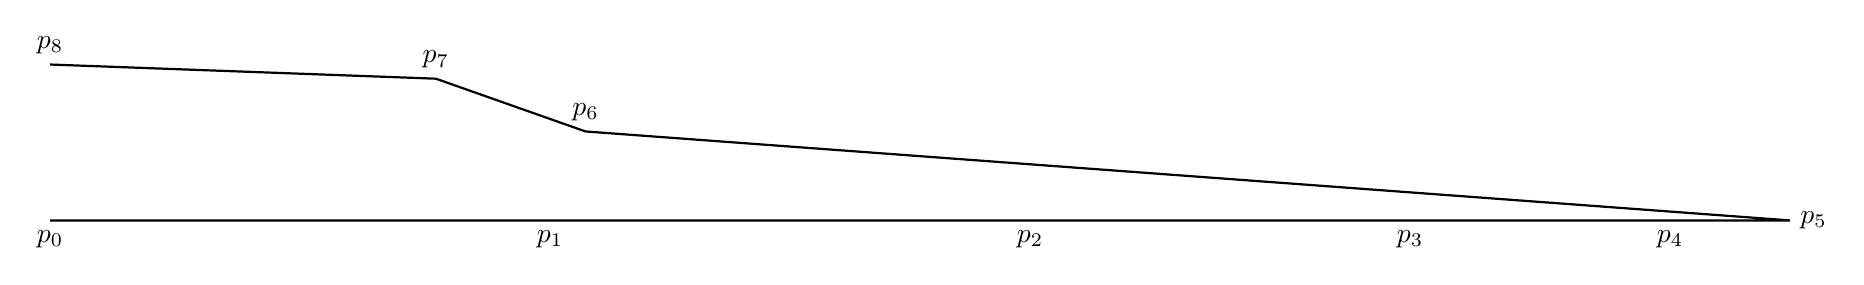
\begin{tikzpicture}

    \coordinate (p0) at \coord(\Cxa,\Cya);
    \coordinate (p1) at \coord(\Cxb,\Cyb);
    \coordinate (p2) at \coord(\Cxc,\Cyc);
    \coordinate (p3) at \coord(\Cxd,\Cyd);
    \coordinate (p4) at \coord(\Cxe,\Cye);
    \coordinate (p5) at \coord(\Cxf,\Cyf);
    \coordinate (p6) at (6.80,1.13);
    \coordinate (p7) at (4.90,1.80);
    \coordinate (p8) at (0,1.98);

    \draw[thick]
           (p0) node[below] {$p_{0}$}
        -- (p1) node[below] {$p_{1}$}
        -- (p2) node[below] {$p_{2}$}
        -- (p3) node[below] {$p_{3}$}
        -- (p4) node[below] {$p_{4}$}
        -- (p5) node[right] {$p_{5}$}
        -- (p6) node[above] {$p_{6}$}
        -- (p7) node[above] {$p_{7}$}
        -- (p8) node[above] {$p_{8}$};

\end{tikzpicture}
\end{document}
